\chapter{State of the Art}\label{STATE}
\smallskip
\hfill
\begin{minipage}[b]{8cm}
{\it Il est tr\`es important, pour celui qui souhaite d\'ecouvrir, de ne pas limiter son esprit \`a un seul chapitre de la
science mais plut\^ot de rester en contact avec plusieurs autres.}
\end{minipage}
\begin{flushright} Jacques Hadamard. \end{flushright}
\vskip 2cm

\section{Terms definition}

\begin{itemize}

\item \textbf{Resilience} \label{resilience} : Being able to defend against an attack as long as
possible, and once the defenses have fallen, being able to return to
nominal execution operation as quickly as possible. In a connected
car, the highest resilience is needed. This resilience is here to
improve the *Security* the car, but without any impact on the *Safety*
because human lifes are involved.

\item \textbf{Security} : The defensive security of an device. This consists in
ensuring the security of an application against hacking and taking
control of that application.  A connected car that involves human
lives and the privacy of these users. It is necessary that the
connected car on which we are going to work has as little *flaw* as
possible, and therefore the smallest possible *attack surface*.

\item \textbf{Safety} : The operational safety of a device. This consists in
ensuring that an object can function properly in a guaranteed
way. That everything goes well when it has to go well. The connected
cars involve human life and are running *safety critical application*, so
we want to be able to guarantee that the car will operate optimally at
all times and that the defense methods used do not break this
assurance.

\item \textbf{Flaw} : Something an attacker can exploit to try and launch his
attack. Can be found by analysing the system operation or analysis the
system code to find any mistakes that could lead to an attack. We want
to avoid as many flaws as possible and/or eliminate existing
ones. With the added defensive methods, make sure that it does not add
new vulnerabilities.

\item \textbf{Attack Surface} : What is visible from a system by an attacker,
and which could be exploited by this attacker in order to find a flaw.
The larger the attack surface of a system, the more likely an attacker
may have a way to try to attack that system. This may help to verify
that the attack surface once the defensive methods have been deployed
has not increased the initial attack surface.

\item \textbf{Safety Critical Application} : Services and applications that are
considered critical. It is therefore necessary to be able to guarantee
certain properties on execution/response time, as well as time
guarantees before failure.  Connected cars have several critical
applications, for which it must be ensured that they remain safe and
protected. Once the new defense methods have been applied to the car,
these defenses must not disrupt the operation of these critical
applications.

\item \textbf{Confidentiality} : The protection of access to all data relating
to the user's private life, habits, travel etc... Because of the
network connections provided to the various connected objects, we do
not want information relating to the privacy of their users to be
disclosed and allow safe use of these objects.

\item \textbf{Integrity} : Ensure that all applications in a system operate
normally. This integrity is due to the defense mechanisms on this
system preventing malfunctions of this one.  If the integrity of the
car is compromised, an attacker can apply the brakes of this car on
the highway, installing malware etc.


\end{itemize}

\bigskip

Resilience is divided into six categories: 

\begin{itemize}

\item Redundancy : Replicate Hardware or software instance inside the
  system to make multiples checks of output or to get a new valid
  instance if one is corrupt

\item Obfuscation : Methods that aim to hide system informations' to an
  attacker. So he will have to investigate and crack the hiding
  methods.

\item Cryptography : Special mathematical obfuscation methods that made
  one way, once use it is extremely difficult to reverse.

\item Monitoring : Checking the integrity of the system with an external
  system looking at the system operation. May be done with redundancy.

\item Authentication : The insertion of data and/or structures to verify
   the integrity or provenance of code, data or hardware.0

\item Isolation : Divide functionality physically or logically and
 controlling interfaces to limit a system’s attack surface, like
 TrustZone in ARM CPU.
 
\end{itemize}
 
Three of the five categories: separation/isolation, obfuscation, and
authentication are for the most part, used to secure a system, i.e.,
to maintain consistency between the perceived system functionality and
the actual system functionality. The other two: redundancy and
monitoring are employed when the operating parameters exceed the
ability of the security techniques to guarantee integrity of the
environment.

\newpage

\section {Moving Target Defense}


{\Huge R}eturn-oriented Programming \emph{(RoP)} attacks~\cite{hund_return-oriented_nodate} unusable\cite{lei_moving_2018, cai_moving_2016, lei_moving_2018, xu_2014}. 
\cite{lei_moving_2018,okhravi_survey_2013, okhravi_finding_2014, lei_moving_2018}:
\cite{noauthor_karl_nodate}
dynamically change the IP address of a system~\cite{ayrault_run_2019}.


The principle of \textbf{Moving Target Defense(MTD)} as seen in
~\cite{okhravi_2014} ~\cite{survey_cyber} ~\cite{lei_moving_2018} is to make an
assymetrically relationship between defender and attacker by
giving the advantage of time to the defender. This is done by
dynamically reconfiguring differents properties of the
platform. \newline
It is necessary, however, that the changeover time be
smaller than that which the attacker needs to realize his
attack. Otherwise this technique is ineffective.

There are 5 categories of moving target defense :

\begin{itemize}

\item \emph{Dynamic Data}. Change the format of data representation.
\item \emph{Dynamic Soft}. Change the code of the application.
\item \emph{Dynamic Runtime Environment}. Change the execution environment.
\item \emph{Dynamic Platform}. Change the properties of the platform.
\item \emph{Dynamic Network}. Change the configuration and properties of the network.
\end{itemize}

Rajouter un paragraphe sur attack surface ?

\subsection{MTD Categories}

\subsubsection{Dynamic Data}

This \emph{MTD}method consists of changing the representation format
data in memory in order to make reading and decoding of different data
stored in memory more complicated because there is no consistency. The
figure \ref{fig:ddata} shows two differents representations format for
the same data. \newline
This method has never been implemented in a system and only served for
research. Using non-uniform data in a file or database renders reading
for the application much harder.


\begin{figure}[h]
  \centering
  \begin{subfigure}{0.49\textwidth} % width of right subfigure
  \centering
    \begin{lstlisting} [ basicstyle=\tiny]
      Age :24
      Gender : Male
      ID : 443
    \end{lstlisting}
    \caption{Format 1}
  \end{subfigure}
  \hfill
  \begin{subfigure}{0.49\textwidth} % width of left subfigure
    \centering
    \begin{lstlisting} [basicstyle=\tiny] 
      ID : 443
      Age :24
      Gender : Male
    \end{lstlisting}
    \caption{Format 2}
  \end{subfigure}
  \caption{Different  data representation}
  \label{fig:ddata}
\end{figure}


\subsubsection{ Dynamic Soft}

The \emph{Dynamic Software}method consist in to have multiple assembly
versions of the same high level code in order to make attacks by
injection of faults, predictions of connections or search for more
fault, more complicated. This is like having code redundancy to a
 behavior less predictable.The figure \ref{fig:dsoft} shows two
code assembler arm equivalent. \newline
This type of method is complicated to integrate in the commercial
area, because it is necessary  to have the source code of the
application available, to be able to compile it with different
options and/or compilers. This option also poses the problem of
performance, a soft is often compiled with options to get
the best performance. Having multiple versions pose the problem that
not all versions would be equally powerful and we would potentially create an
overhead.


\begin{figure}[h]
  \centering
  \begin{subfigure}{0.45\textwidth} % width of right subfigure
    \centering
    \begin{lstlisting} [ basicstyle=\tiny]
      add r5, 0, 0
      add r3, 0, 3
      lsl r5, r3
    \end{lstlisting}
    \caption{Code 1}
  \end{subfigure}
  \hfill
  \begin{subfigure}{0.49\textwidth} % width of left subfigure
    \centering
    \begin{lstlisting} [ basicstyle=\tiny]
      xor r5, r5, r5
      xor r3, r3, r3
      add r3, r3, 8
      mul r5, r5, r3
    \end{lstlisting}
    \caption{Code 2}
  \end{subfigure}
  \caption{two equivalent assembly code}
  \label{fig:dsoft}
\end{figure}


\subsubsection{ Dynamic Runtime Environment}


The \emph{Dynamic Runtime Environment}is a method that consist in modify
the execution environment of the application in order to prevent that the
attacker directly access certain zone of memory or instructions
flow. This method encompasses two sub methods, the \emph{Address Space
  Layout Randomization (ASLR)} and the \emph{Instruction Set Randomization(ISR)}. \emph{ASR}
is the most used method in real cases. It is include inside almost all
the commercial OS. 

The \emph{ASLR}makes random the layout of the virtual memory of the
program at the time of its execution. This can change the base
address of different segments like stack, heap, libraries
sharing... in order to make it more difficult to spot.
These changes are usually directly done by
modifying the kernel the OS uses.  \newline
However this method is not very effective on small
memory. The time to try in brut force becomes very short, and
it does not bring much more defense.

The \emph{ISR}makes random the current instruction of an application. By
example by encrypting each instruction when loading
these and decrypting it at the time of execution. This makes more
difficult to exploit memory vulnerabilities.
With ISR, code injected by attackers will not be properly encoded but
still go through the decoding process. This leads to illegal CPU
instructions and exceptions.

There is also the System Call Number Randomization (SCNR) that can be
use for Dynamic Runtime Environement MTD. The principle of this
technique is related to the ISR, here we randomize the number of the
System Call instead of the instruction. So when there is code
injection the system call leads to an error or a different result as
expected.

in this online web site ~\cite{daniel_2017}, we can see the difference
between \emph{ASLR}, \emph{KASLR} and \emph{KARL} . We already spoke about \emph{ASLR}, so
we will focus on \emph{KASLR}and \emph{KARL}. \newline
In \textbf{KASLR} (\emph{Kernel Address Space Layout Randomization}), we randomize the
kernel code location when the system boots. It was introduced in the
linux kernel in 2014, and has been enable by default since 2017. But
it's effectiveness is questioned because until the next
system reboot, there will be no other new random distribution in the
memory. \newline
 \textbf{KARL} (\emph{Kernel Address Randomized Link}) ~\cite{karl} has been recently
released in OpenBsd, and not based on ASLR. With this, the kernel is
still located in the same addresses of the KVA (Kernel Virtual Address
Space), but this time, every time the system is reboot or updated, the
kernel binary files are randomize. So each time the system is boot, we
have a unique kernel totaly different from other system at binary
level. In ~\cite{rekarl} we can see the difference between the BSD kernel code
with and without the Karl system. It is said in those links, that it
took around 1 second on a fast machine for the entire BSD kernel, for
a small car kernel it should take less than that.


\subsubsection{ Dynamic Platform}


This method consists in changing the properties of the platform on
which the application is running to prevent attacks based on a specific
architecture. This technique is based on the change, for example, of
the OS, the processor architecture, virtual machine instance, file
system, communications ... It also proposes to migrate an application
of one platform to another in order to avoid having persistent attack.

This method is more useful for server based system, there is technique
like temporal changes (virtual machine rotation) or diversity
(multiple variant execution). This means that we have per example
multiple redundant servers with different softwares running on it (like
Apache or IIS server). It will increase the availability of the
service and make it more difficult to attack.

\subsubsection{Dynamic Network}

This method consists of changing the configuration and properties
associates with the network of the platform. The principle of this
method consists in regularly changing the IP addresses, the open ports
of comunication as well as the topology of the network. This allows to
slow down the attacker's appreciation before he starts to try to
access the machine.

By changing the table title of a database periodicaly, this could slow
down SQL injection without causing failure in the system. With IP
randomization, the IP address is changed periodically and
the  communication of  the new address is only  for authorized user. This will
reduce attacker's capabilities to scanning or exploiting the
system. And if the system receive some request from the outside, it
will communicate fake informations, like the OS version, the
application identity.

We can combine this technique with \emph{Honey Pots}dynamically changing
of location, in order to confuse the attacker. \emph{Honey pots}generally
consists in letting some data, ports or anything open that appears
legitimate to the attacker, but is actually isolated and monitored,
and seems to contain valuable information. So the attacker thinks to
be in the system and have acces to data but he is not. While moving dynamically
 the honey pot, the attacker can never knows if he is really in or it is just
 a honey pot.

\subsection{Measuring the effectiveness}


There is three big group of measurement approaches of MTD efficiency,
\emph{Attack based Experiments}, \emph{Probability Model} and \emph{Simulation-based}
Evaluation. 

The first one, the \emph{Attack-based Experiments} evaluate an MTD method
how much it is difficult to compromise a program. It is use directly
on a system with some MTD method running. So we can measure the time
we need to access to the system with and without MTD and conclude if
the method used is effective against some attacks and produce better
results than the system without MTD.

The Second one is the \emph{Probability Model}. In this one we analyze
attacking success when MTD are use. We have to build a probability
model of out system. In this model we abstract the specificities of
the system, the attacks and the defenses instance as probability. By
example the length of the randomization key of ISR is represented as a
variable related to the probability of a successful attack. \newline
Because of the abstraction, we might be missing some key informations,
and get at the end a mismatch between the model and the reality.

There is next the \emph{Simulation-based Evaluation}. In this, we launch
periodically some attacks of an attack graph predefined on some system
with a MTD technique deployed on it. \newline
The success of an attack is determined by a pre-defined probability
model and a specific MTD implementation. Results of the simulation
quantify the relationship between successful attacks and different
MTD settings (like frequency of diversification). In their settings,
for instance, the ratio of successful attacks is 50\% when MTD is
\emph{switch off}which goes  to 15\% if we \emph{switch ON}the MTD. \newline
With a simulation-based approach, a whole system can be abstracted as
numeric parameter, and there is no restriction on the specifics of
attacks and defenses. A simulation-based method provides people
with a uniform approach to evaluate MTD techniques with the least
effort.

So we can define attack-based approaches as low level methods, and the
two other as high level method. \newline 
Low level method permit to see what happen directly inside a function
or application so we can have results with very high accuracy. But it
is difficult to compare MTD only on evaluation through attack-base
experiments. We only have results for the program context that can not
be use directly as comparable metrics. A low-level method works at the
scope of an individual program.  When used in a system with multiple
interconnected programs, a low-level method is limited. Such
limitations are caused by the absence of a model for interaction
between different programs. Attack effects that propagate through
program interactions could not be captured by a low-level
method. \newline
In the other hand, high level methods permit to
see the system as a black box. But low levels contexts are abstract or
neglected, so it is difficult to reflect what really happens in a
system.

\subsubsection{ First approach}

So far from now, there is not any method that permit to fill the gap
between the two methods. XU and al.~\cite{xu_2014} tried to fill this gap
with an other method in three layers that permit to compare different
MTD methods in a system.

The \emph{first layer}is use to describe each application with a \emph{State
Machine}so we can have use the low levels methods to see any
problems inside an app under attack. So we get after that the \emph{second
layer}that work to make interaction between all applications. So if
one is compromise and affect an other we will see. This \emph{High Level Methods}
is use in this case. Then we have the \emph{third layer}that put
everything together and permit to an user to see how the system is
compromise, and how the attack have develop in it. \newline 
With this method it is possible to compare different MTD method to
find the best one for our system.


\subsubsection{ Second approach }

In this approach ~\cite{moody_2014} they tried to use \emph{Stochastic Petri
Nets}to evaluate the effectiveness of the MTD technique used to
defend in a distributed application environment. A Stochastic Petri
Nets is a petri net in which on each transition we have a time. This
time corresponds to a delay between enabling the transition and taken
it. \newline First they build a model of their system without MTD with
Stochastic Petri net so they can see how many time it takes to attack
the system, then they build an another Stochastic Petri net of their
system but with MTD this time, to see if the attacker makes more time
to get into the system than without the MTD.


\subsubsection{ Third approach }

In this paper, Carroll and al ~\cite{carroll_2014}, they used probabilistic
model and simulation calculate the effectiveness of network address
shuffling. \newline The probabilistic model used in this etude is the
urn model. It is a simple model in which we consider that we have a
bag with marbles in it. We have got two kind of marbles, green one and
blue one. The green one represents the IP addresses that are not valid
or not used by our system. And the blue one the IP addresses used and
vulnerable by our system. We have $n$ blue marbles and $m$ green
marbles.\newline So every time the attacker scan the network for
vulnerable IP addresses, we consider that he pick $k$ marbles, if in
those marbles he get at least one blue marble, then he has something
to attack. In the configuration without MTD, the number of marbles in
the bag keep to decrease at every pick, and after a certain time, the
attacker will have all the marbles. But if we use perfect MTD that
shuffles IP addresses every time after every probe, then we put back
every marble in the bag after every time the attacker scan the
system. So the attacker will make more time to get the vulnerable
entry. With this method and formula in the paper, we can get a model
to test the efficienty of a MTD.

In this other paper, Luo and al ~\cite{luo_2014} tries this time with the
same method (urn model) to evaluate the efficienty of port
shuffling. And they get to the same conclusion.


\subsubsection{ Forth approach}

This approach made by Clark and al ~\cite{clark_2013} intented to calculate
the effectiveness of IP Address randomization in a \emph{decoy-based MTD}
with a model of the interaction between adversary and defender.
\newline In a decoy-based MTD, we introduce some decoy nodes in the
system, each node gets a valid IP address with a tiny protocol to respond
to requests and mimic a real node. Then we take all node the real
and the decoy and we randomize periodicaly the IP addresses, in order
to reduce the probability that the attacker discovers the real
node. They present their study with a Matlab model of this simulation
to get if the decoy based MTD model is effective or not. The model is
based on simulation of the model with probabilities.


\subsection{ Different way to measure effectiveness}

An other way to measure the effectiveness of a MTD technique is to use
\emph{Attack Graph}An attack graph is a graph in which we represent a
succession of steps the attacker needs to perform in order to access
to some privileges on the system. With this to it exists two metrics,
one only by examine the graph, and the second by add some more inputs
to the graph. Each of them have pros ans cons.

\subsubsection{ Graph only}

There exist some methods to measure the effectiveness of an MTD
technique only with \emph{attack graph}.\newline
The first one describe in ~\cite{phillips_1998} consist in looking for the
smaller path in the graph to get access to some privilege. So the
longer this path is the more secure the system is. But there is
limitation to use only this technique, we can not make difference
between two system with the same smaller path length, with one that
got only one path and the other that got more. \newline
A second technique describe in ~\cite{li_2006} is about compute the average
length path in the graph. It may be useful when we have two smalls
graphs of almost the same sizes. Otherwise we can get false or not
trusty results. \newline
A third one describe in ~\cite{Ortalo_1999} is about counting the number of
path that leads to a privilege access. The more one got, the more it
is un secure. But here we don't look at the difficulty to get through
the path. You can have only one but really easy to follow, or a bunch
and very difficult to access.

\subsubsection{Graph plus input data}

The key of this techniques is to add probability to each node of the
graph to represent the difficulty to pass by. So with this adding to
an attack graph we can get a better understanding of the difficulty to
follow a path to a vulnerability.

~\cite{noel__2010}
 
\subsection{ Attack Timeline}

 the attack timeline can be seen as 5 different phases. Each phase has
a purpose during the attack, and each MTD category intend to counter
one or more of the attack phases. \newline
The first one is \textbf{Reconnaissance} in which the attacker try to find the system on the
network, like example scanning the IP address around him to locate it,
or trying to find the open ports of the system. So if we counter this
first phase the attacker will not be able have access to the
system. \newline
The second one is \textbf{Access} in which the attacker try to break into
the system by a leak he has found during the first attack. Most of the
time this is possible because he knows the architectural platform and
all the possible breach. \newline
The third one is the \textbf{Development} phase in which the attacker
deploy his malicious code in the application he have now access to. We
have seen that almost all the MTD categories can counter this one by
various methods. \newline
The fourth one is the \textbf{Launch} phase in which the attacker give the
command to the system to launch his attack, and in which the system
will probably encounter faults. It is possible to get here once he has
access to the system and has already deployed his
malicious code. \newline
And finally the last one, the \textbf{Persistence} phase in which the
attacker tries to leave a backdoor open for the next time he wants to
break in the system. \newline 
The table~\ref{tab:my-table} describe, which MTD category is effective against
which phase of the attack.

\begin{table}[h]
  \centering
  \begin{tabular}{llllll}
    MTD/attack                       & Reconnaissance & Access & Development & Launch & Persistence \\ \hline
    \multicolumn{1}{l|}{Network}     & \checkmark     &        &         & \checkmark &        \\
    \multicolumn{1}{l|}{Platform}    &          & \checkmark   & \checkmark &       & \checkmark    \\
    \multicolumn{1}{l|}{Runtime Env} &                &        & \checkmark           & \checkmark      &             \\
    \multicolumn{1}{l|}{Software}    &                &        & \checkmark           & \checkmark      &             \\
    \multicolumn{1}{l|}{Data}        &                &        & \checkmark           & \checkmark      &            
  \end{tabular}
  \caption{MTD effectiveness against which attack phase}
  \label{tab:my-table}
\end{table}

In order to get the best protection during all the attack, we need to
combine multiple MTD techniques to be the safest possible.




\newpage
\section {Game Theory}

\subsection{Presentation}



{\Huge L}a th\'eorie des jeux est la science de la prise de d\'ecision strat\'egique. La th\'eorie des jeux a \'et\'e utilis\'ee dans des sciences aussi diverses que la biologie \'evolutionniste, le management des d\'ecisions (politique) et l'\'economie. Elle peut \^etre d\'efinie comme l'\'etude de mod\`eles math\'ematiques des conflits et coop\'erations entre d\'ecideurs intelligents et rationnels.
La th\'eorie des jeux fournit des techniques math\'ematiques g\'en\'erales pour analyser des situations dans lesquelles deux personnes ou plus prennent des d\'ecisions qui s'influencent mutuellement.

Dans le langage de la th\'eorie des jeux, un jeu fait r\'ef\'erence \`a toute situation impliquant deux sujets ou plus. Les sujets impliqu\'es dans un jeu peuvent \^etre appel\'es les \emph{joueurs}. Comme indiqu\'e dans la d\'efinition ci-dessus, il y a deux hypoth\`eses de base que les th\'eoriciens des jeux font g\'en\'eralement \`a propos des joueurs: ils sont rationnels et intelligents. 
Chacun de ces adjectifs est utilis\'e ici dans un sens technique qui n\'ecessite quelques explications. Un d\'ecideur est rationnel s'il prend des d\'ecisions de mani\`ere coh\'erente de ses propres objectifs. En th\'eorie des jeux, en s'appuyant sur le fondamental r\'esultats de la th\'eorie de la d\'ecision, nous supposons que l'objectif de chaque joueur est de maximiser la valeur attendue de son propre gain, qui est mesur\'e en une certaine \'echelle d'utilit\'e. L'id\'ee derri\`ere un \emph{d\'ecideur rationnel} est que les actions s\'electionn\'ees (nomm\'ees \emph{strat\'egies}) maximiseront les b\'en\'efices d'utilit\'e attendus par le joueur. Cette id\'ee remonte au moins \`a Bernoulli (1738), mais la justification moderne de cette id\'ee tient \`a Von Neumann et Morgenstern (1947) ([xx]).

Many decision problems can be modeled using game-theoretic concepts, with
applications to various domains, reaching from program synthesis to resource
allocation in smart grids. Games are a natural model for security problems: They
allow to formalize the goals of potential attackers in terms of objectives of an
adversarial player, and provide a mathematical framework to reason about defense
strategies. 
The use of game theory~\cite{prisner_game_2014} provides a representation of the problem posed in the form of an optimization problem.

In general, in a mathematical game, each player chooses from a set of available \emph{actions}. The choice of actions of the different players can be done in different ways corresponding to two basic categories of games:
\begin{itemize}
	\item \textbf{Simultaneous games} in which the players choose their respective actions at the same time without knowing in advance the choices of the other players.
	\item \textbf{Sequential games} in which the players are playing in a (fixed) order, such that all other players can observe the first player's action before taking a decision.
\end{itemize}

Choosing an action to perform results in a \emph{reward} that could be more or less attractive depending on the adversary's choice.
The payoffs of choosing an action for the different players are defined in terms of \emph{reward functions}: The value of the payoff depends on the combination of actions chosen by the different players. The most common way to represent reward functions is by a matrix (see for example Table~\ref{tab:normalform}), called the \textit{normal form}. In this example, the attacker has the choice to attack or not to attack and the defender to defend or not to defend.  For each combination of actions, the table gives a pair of constants, corresponding to the reward for each player: $r_a$ for the attacker and $r_d$ for the defender.

\begin{table}[h]
    \centering
    \caption{Attacker/defender normal form game \label{tab:normalform}}
    %\label{Tab:table1}
    \begin{tabular}{l|l|l}
                & Defend               & Not Defend           \\ \hline
     Attack     & $(r_{a1}$, $r_{d1})$ & $(r_{a2}$, $r_{d2})$ \\ \hline
     Not Attack & $(r_{a3}$, $r_{d3})$ & $(r_{a4}$, $r_{d4})$
    \end{tabular}
\end{table}



\subsection{General Definition}
Pour expliquer les concepts de la th\'eorie des jeux, prenons un exemple; "\emph{l'\'evitement de la congestion du r\'eseau internet}". Le r\'eseau internet est bas\'e sur le protocole TCP/IP. En TCP/IP, un fichier est d\'ecoup\'e en paquets qui transitent entre les diff\'erents noeuds du r\'eseau entre l'\'emetteur et le r\'ecepteur. Chaque fois que le r\'ecepteur re\c{c}oit un paquet, il envoie un accus\'e de r\'eception \`a l'\'emetteur. De cette fa\c{c}on, le l\'emetteur sait que le paquet est bien arriv\'e. Le protocole TCP/IP cherche \`a augmenter le d\'ebit du r\'eseau jusqu'\`a sa saturation. Lorsque l'un des noeuds du r\'eseau est satur\'e, il efface des paquets jusqu'\`a d\'esaturer. L'\'emetteur ne recevant plus d'accus\'e r\'eception pour un paquet va le r\'e-\'emettre apr\`es une certaine temporisation (g\'er\'e par l'algorithme d'\'evitement de congestion). Si tous les \'emetteurs suivent cette r\`egle, cela  permet de d\'esaturer le noeud pour le b\'en\'efice de l'ensemble des utilisateurs. Cependant, il est possible pour certains \'emetteurs de violer cette r\`egle et de r\'e-\'emettre le message sans latence. 

Ce comportement peut \^etre mod\'elis\'e en th\'eorie des jeux.  Imaginons, deux personnes utilisant Internet. Elles ont deux choix possibles\ :
\begin{itemize}
\item Utiliser la version correct de l'algorithme d'\'evitement de congestion du r\'eseau. Cette strat\'egie est not\'ee \emph{C}.
\item Utiliser une version d\'efectueuese de l'algorithme d'\'evitement de congestion du r\'eseau. Cette strat\'egie est not\'ee \emph{D}.
\end{itemize}

Le comportement du r\'eseau est le suivant; si les 2 personnes choisissent la strat\'egie \emph{C}, chaque paquet sera retard\'e de 2ms. Si les 2 personnes choisissent la strat\'egie \emph{D}, chaque paquet sera retard\'e de 4ms. Si une des personnes choisit l'action \emph{C} et l'autre l'action \emph{D}, le premier voit ses paquets retard\'es de 6ms et le second voit ses paquets re\c{c}us sans retard. Bien s\^ur, chaque personne est rationnel et cherche \'a augmenter son d\'ebit, c'est \`a dire dans notre exmple, \`a minimiser le retard de ses paquets.

\subsection{Game representation}

\begin{defn}
Un jeu peut \^etre mod\'elis\'e par un triplet $<N, S, u>$ avec:
\begin{itemize}
\item N repr\'esente les joueurs. $N = \{1,2,\ldots,n\}$ est un ensemble de cardinal $n$ (nombre de joueurs dans le jeu). 
\item $S$ repr\'esente l'ensemble des combinaisons de strat\'egies possibles pour l'ensemble des joueurs $S: S_1 \times S_2 \times \ldots \times S_n$ avec $S_i$ l'ensembles des strat\'egies possibles pour le joueur $i$. Tous les joueurs n'ont pas n\'ecessairement les m\^eme strat\'egies et certaines combinaisons de strat\'egies peuvent \^etre impossibles. 
\item $u$ repr\'esente la fonction de $u: S \to \R^n$ qui associe \`a chaque combinaison de strat\'egie une valeur d'utili\'e avec pour chaque $u_i$\ :
  \begin{itemize}
  \item une valeur n\'egative repr\'esentant une perte pour le joueur $i$
  \item une valeur positive repr\'esentant un gain pour le joueur $i$
  \end{itemize} 
\end{itemize}
\end{defn}

Il est plus commode de repr\'esenter la fonction d'utilit\'e pour le joueur $i$ comme $u(s_i, s_{-i})$, avec 
$s_{-i} = (s_1, s_2, \ldots, s_{i-1}, s_{i+1}, \ldots, s_n)$ qui repr\'esente la strat\'egie jou\'ee par tous les autres joueurs et de noter $u_i$ la i-\`eme composante de la fonction d'utilit\'e.
\\

Pour notre exemple, nous avons:
\begin{itemize}
\item 2 joueurs, $N = \{1,2\}$
\item les strat\'egies possibles pour les 2 joueurs sont identiques $S_1 = S_2 = \{C,D\}$. Et l'ensemble des combinaisons de strat\'egies possibles est d\'efini comme $S=\{(C,C),(D,C),(C,D),(D,D)\}$
\item la fonction utilit\'e peut \^etre repr\'esent\'ee par la matrice suivante\ :
\end{itemize} 

\begin{center} 
\begin{tabular}{|c||c|c|}
\hline 
\diagbox{$Joueur_1$}{$Joueur_2$}  & $C$ & $D$ \\ 
\hline \hline
$C$ & (-2,-2) & (-6,0) \\ 
\hline 
$D$ & (0,-6) & (-4,-4) \\ 
\hline 
\end{tabular}
\end{center}

\subsection{Strategie}
\subsubsection{Dominance}

Intro Dominance

\begin{defn}
Une strat\'egie $s^{*}_{i}$ \emph{domine strictement} (strictly dominates) la strat\'egie $s_i$ ssi\ :
$$
\forall s_{-i} \in S_{-i}, u_i(s^{*}_{i}, s_{-i}) > u_i(s_{i}, s_{-i}) 
$$
\end{defn}

Quelque soit ce la strat\'egie choisie que les autres joueurs, la strat\'egie $s^{*}_{i}$ est le meilleur choix pour le joueur $i$. Comme le joueur $i$ est rationel, il ne va jamais jouer une strat\'egie domin\'ee $s_i$. 

\begin{defn}
Une strat\'egie $s^{*}_{i}$ \emph{domine faiblement} (weakly dominates) la strat\'egie $s_i$, ssi
$$
\forall s_{-i} \in S_{-i}, u_i(s^{*}_{i}, s_{-i}) \geq u_i(s_{i}, s_{-i}) 
$$
et
$$
\exists s_{-i} \in S_{-i}, u_i(s^{*}_{i}, s_{-i}) > u_i(s_{i}, s_{-i})
$$
\end{defn}

Quelque soit la strat\'egie choisie par les autres joueurs, la strat\'egie $s^{*}_{i}$ est au moins aussi bonne que la strat\'egie $s_i$ pour le joueur $i$. 


Il est maintenant possible d'\'etendre ces d\'efinitions sur l'ensemble des strat\'egies possibles pour le joueur $i$.

\begin{defn}
Une strat\'egie $s^{d}_{i}$ est \emph{strictement dominante} (resp. \emph{faiblement dominante}) pour le joueur $i$ ssi $s^{d}_{i}$ domine strictement (resp. domine faiblement) toutes les autres strat\'egie pour le joueur $i$.
\end{defn}

Pour notre exemple, pour le joueur 1, la strat\'egie $D$ domine strictement la strat\'egie $C$. En effet, on a $S_{-1} = \{C, D\}$. pour $s_{-1} = {C}, u_1(D, C) > u_1(C, C)$ et pour $s_{-1} = {D}, u_1(D, D) > u_1(C, D)$. En fait, la strat\'egie $D$ est \'egalement la strat\'egie strictement dominante pour le joueur 2.

Comme le joueur $i$ est rationnel, et qu'il existe une strat\'egie strictement dominante, alors le joueur $i$ ne va pas jouer une autre strat\'egie.

\subsubsection{Pure Strategie}

Une fois trouvé une stratégie peut être de deux formes, pure ou mixed.

Une stratégie pure correspond à une stratégie dans laquelle chaque joue choisit un et un seul mouvement à réaliser qui sera choisit à coup sûr.

Pour la strétégi

\subsubsection{Mixed Strategie}

\subsection{Types of game}

\subsubsection{Simultaneous Game}

\subsubsection{Turn by turn Game}

\subsubsection{Bayesian Game}

A Bayesian game~\cite{paruchuri_efcient_nodate} is represented by a set of players $G$ in which each player $g$ must be of a given type of the set of type $\theta_g$. In this work, the games we consider have two players: the defender $d$ and the attacker $a$. While there is only one type of defender, $\theta_a$ contains as many elements as there are attackers. 
During the game, the attacker knows her own type, but it is unknown to the defender. A probability distribution $\gamma$ defines the probabilities for each of the players of being of a specific type. Note that the type is chosen once before the game starts.

Each player $g$ has a finite set of available actions $A_g$. The reward for each player then depends on the actual type of the players and the chosen actions:  $R_g : \theta_d \times \theta_a \times A_d \times A_a \rightarrow \mathbb{R}$ for $g \in \{a,d\}$.

There exists a way to transform a Bayesian game to normal form thanks to the transformation of Harsanyi~\cite{harsanyi_generalized_1972}. This allows us to find a solution to this problem through a linear program for finding the best possible existing strategy. 


\subsubsection{Stochastic Game}

\subsubsection{Dynamic Game}

\subsubsection{Learning Game}


\subsection{Game resolution}

\subsubsection{Nash Equilibrium}

\subsubsection{Stackelberg Equilibrium}

\subsubsection{Harsanyi Transformation }

\subsubsection{Complementary slackness}

With the complete explication after presenting the Stackelberg equilibrium and harsanyi transformation, that can be useful with some type of game Stackelberg + Bayesian.


The search for an optimal strategy gives rise to an optimization problem. In some cases, it can be efficiently solved using for example linear programming. 

% In linear optimization, we search for an optimal solution to a problem represented in the form of a mathematical model that allows us to maximize one of the output parameters such as the maximum profit that can be obtained by performing an action, or the minimum cost that can be reached when producing an object.

In general, a linear program is represented by an objective function to maximize, and a set of constraints, such as presented in the equation below. Here, $x$ corresponds to a vector of variables we are trying to determine,  $c$, $b$ are vectors, and $A$ is a matrix.

\begin{flalign}
&\max_{x} c^T * x \label{primal} \\
&\text{Where: } A x \leq b \nonumber\\\
&\text{and: } x \geq 0\nonumber 
\end{flalign}

This is also called the \emph{primal} of the problem. It can be rewritten in another way, in order to try to find an equivalent solution, called the \textit{dual} of the problem presented in \ref{form:dual}. Here, $y$ corresponds to the variable we are trying to determine, and $c$, $A$ and $b$ are the same elements as in the primal.

\begin{flalign}
& \min_{y} b^T * y \label{form:dual} \\ 
& \text{Where: } A y \geq c \nonumber\\
& \text{and: } y \geq 0 \nonumber 
\end{flalign}

In order to show that we have found an optimal solution to the original problem, we must verify the \emph{complementary slackness} which says that if $x_0$ is a solution to the primal and $y_0$ is a solution to the dual, and that $c^T * x_0 = b^T * y_0$ then $x_0$ and $y_0$ correspond to the optimal solution of the problem.

In our model, complementary slackness will be added as a constraint in order to force the attacker to choose an optimal solution. This reflects the fact that we assume a rational attacker.


\subsection{DOBSS}

\newpage
\section {Risk Analysis}



\subsection{Attack tree}

{\Huge A}ttack trees are here to help us to provide a formal way of modelling
the security of systems. So the attacks are represent in a tree
structure, with the goal to achieve as root node and the different
paths to complete this goal as leaf node. As describe un example in
figure \ref{attack}. All child are connected to the father with an
\textbf{or} connection except if an \textbf{and} instruction is explicitly
written. \newline
It is also possible to add the label \emph{possible}/\emph{impossible} to each
node. This label is here to say if an action is possible or not to
realize, so it will eliminate some path inside the tree. \newline
The cost to realize some node can be added to in order to help find
the costless path to realize some actions. \newline
To summarize, it is possible to add all kind of label to nodes in
order to add information inside the tree to help analyse it.

\begin{figure}[h]
    \centering
	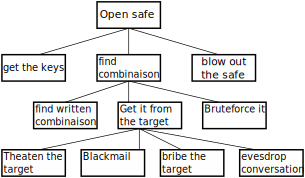
\includegraphics[width=0.55\textwidth]{schema/attack_tree.pdf}
    \caption{Attack Tree example}
    \label{attack}
\end{figure}

Attack tree is a 3-tuple $AT = \{N, C, L\}$ where :

\begin{itemize}

\item $N$ is the set of all the existing nodes with their name.

\item $C$ are the connections between nodes, it describe how each nodes
  are connected to each other like this $\{node_1; node_4; node_9\} \rightarrow
  node_5$

\item $L$ represent all the label that can be attributes to a node.

\end{itemize}

\subsection{Fault tree}

Fault trees in contrary of attack tree is used to represent safety
fault that can occurs inside a system, and to check the different
consequences those errors can lead to. They are represent as a tree
where all node are connected to each other with logical gates. So this
representation is done with DAG, that have two types of nodes, \emph{event}
and \emph{logical gates}An example fault tree is shown in the figure
\ref{fault}\newline
An \emph{event}node represent a failure that can occur in the system or
the failure of a component. Those event are divided into basic event
(BE) that occur spontaneously, and intermediate event (IE) that are
caused by other event. The event at the top of the tree is call the
top event (TE) and is the one that is analyse inside the fault tree.

\begin{figure}[h]
    \centering
	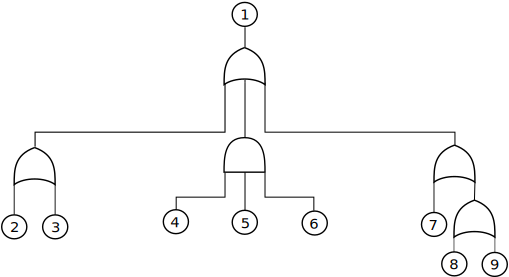
\includegraphics[width=0.5\textwidth]{schema/fault_tree.pdf}
    \caption{Fault Tree example}
    \label{fault}
\end{figure}


Fault tree is a 4-tuple $FT = \{E, G, T, C\}$ where :

\begin{itemize}

\item $E$ represent the set of all the existing event of the tree.
  
\item $G$ represent the set of all gates that exist on the tree.
  
\item $T$ represent the type each gate can take.

\item $C$ represent the connection between gate and events.

\end{itemize}
    
\subsection {(Dynamic) Reliability Block Diagrams (D)RBD}

\subsubsection{Reliability Block Diagrams}

Block diagrams are a way to represent a system by using blocks. Each
component of the system is represented as a block connected, either
directly or in parallel. An example of RBD is shown in Figure
\ref{RDB}. \newline
Each of these blocks is subdivided into smaller blocks that represent
the behavior of the component. Each block contains a failure rate
associated with it. \newline
An RBD can be represented as a logical formula in which the blocks in
series are connected by \emph{and}and the blocks in parallels by \emph{or}.

\begin{figure}[h]
    \centering
	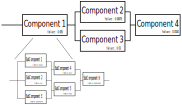
\includegraphics[width=0.65\textwidth]{schema/RDB.pdf}
    \caption{Reliability Block Diagram example}
    \label{RDB}
\end{figure}

Each block is represent like this $B_i\{L\}$ where $_i$ represent the
identifier of the block and $L$ the probability of failure associated
to this block.

Each block can be decompose into a block diagram so as example $B_i =
B_{j} \wedge (B_{k} \vee B_{l}) \wedge B_{m}$

So a RBD is represent by a succession of Block link with each other by
$and$ and $or$ gates.


\subsubsection{Dynamic Reliability Block Diagrams}

Dynamic Reliability Block Diagrams are static ones in which some new
\emph{special}block have been added to make the behaviour of the system it
represents dynamic. Those blocks are SDEP (State Dependency) block,
Spare block, LSH (Load Sharing) block, SEQ (Sequential) block and PAND
(priority) block. \newline

\textbf{SDEP block}are used to model the dependency between multiple
state. Each state affect to it can send and receive 3 type of signal
from this block. $A$ for \emph{Active}, $D$ for \emph{Deactivation} and $F$ for
\emph{Failure}It is used to have a reaction or dependency between
state. If one become activate, one other can be deactivate. By the
same way it is possible to represent the reaction to a system if one
component fails. This is shown in figure \ref{sdep}.

\begin{figure}[h]
    \centering
	\includegraphics[width=0.35\textwidth]{schema/sdep.pdf}
    \caption{SDEP Block example}
    \label{sdep}
\end{figure}


\textbf{Spare block}are here to model the behaviour of the redundant
component. The primary component can send a $D$ or $F$ signal to the
Spare block that will send $A$ signal to different subcomponent. So
the order of usage the redundant component can be modelize. This is
shown in figure \ref{spare}.

\begin{figure}[h]
    \centering
	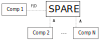
\includegraphics[width=0.35\textwidth]{schema/spare.pdf}
    \caption{Spare Block example}
    \label{spare}
\end{figure}


\textbf{LSH block}are here to help to share the load over the multiple
component. This block get two variable $k$ and $n$ which represent
respectively the minimum number of active component connect to it, and
the total number of component connect to it. So if there is k active
component connect to this block and one become deactivated or fail,
then this block will send a $D$ signal to every other component
connect to it. This is shown in figure \ref{lsh}.

\begin{figure}[h]
    \centering
	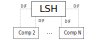
\includegraphics[width=0.35\textwidth]{schema/lsh.pdf}
    \caption{LSH Block example}
    \label{lsh}
\end{figure}


\textbf{SEQ block}are used to specify the order in which some event can
happened between the component connect to it. So it is possible to say
that \emph{component 1}must fail before \emph{component 2}can fail too. In
other way, the \emph{component 2}can't fail before \emph{component 1}fails.

\textbf{PAND block}are used to modelize the occurrence order of some
components. It can be used for this kind of example : If a primary
component is connect to a switch controller as well as a redundant
component. If the primary component fail and the switch is still alive
the redundant component can be activated, but if the primary component
and the switch failed, the redundant component can not be activate and
the system fails.

All those new blocks are used to make the behaviour of a RBD system
dynamic. An example system is shown in figure \ref{DRBD}

\begin{figure}[h]
    \centering
	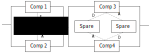
\includegraphics[width=0.65\textwidth]{schema/drbd.pdf}
    \caption{Dynamic Reliability Block Diagram example}
    \label{DRBD}
\end{figure}

\subsection{Boolean logic Driven Markov Processes (BDMP)}

Boolean logic Driven Markov Processes are here to help make fault tree
more dynamic by the addition of Trigger Markov Process. So the basic
concept of it is that every leaf of the fault tree does not represent
any more some basic fault event that could occurs but a Trigger Markov
Process. One Example of a BDMP is shown in figure \ref{bdmp}.

\begin{figure}[h]
    \centering
	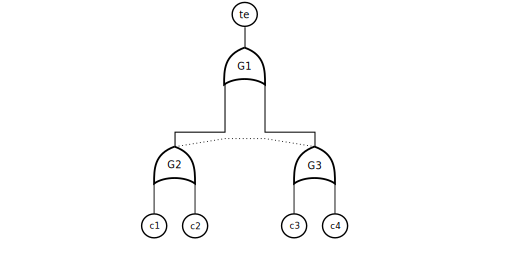
\includegraphics[width=0.75\textwidth]{schema/BDMP.pdf}
    \caption{BDMP example}
    \label{bdmp}
\end{figure}


So Each TMP are composed of four states, Standby, Faulty during
Standby, Working and Faulty during Working, and gets two boolean
variable \emph{Activation Status} and Failure Status. One example can be
seen if figure \ref{tmp}. \newline
So those four states models 2 Markov Chain, one for the behaviour of
the Working state of the component and one for the behaviour of the
standby state of the component. It is possible to  go from one to the
other. \newline
The trigger event represent with a dash line from G2 to G3 leans that
when the output of G2 is True the part the of the system related to
G3, c3 c4, are required. And is the output is False then they are not
required.

\newpage

\begin{figure}[h]
    \centering
	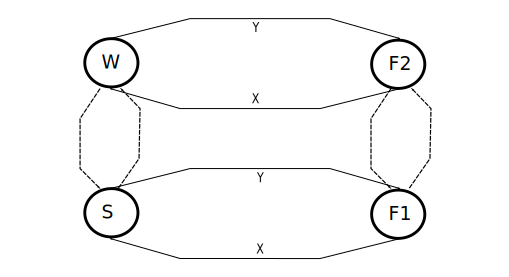
\includegraphics[width=0.5\textwidth]{schema/TMP.pdf}
    \caption{TMp example}
    \label{tmp}
\end{figure}


\subsubsection{Boolean logic Driven Markov Processes formalism}

Boolean logic Driven Markov Processes are a 3-tuple $BDMP = \{FT, TMP, Tr\}$ where :

\begin{itemize}

\item $FT$ represent the Fault Three.

\item $TMP$ represent the set of all TMP associated to each leaf of the fault tree.

\item $Tr$ represent the set of triggers

\item $te$ represent the top-event of the fault three

\end{itemize}

\subsection{CVSS}


\textbf{Common Vulnerability Scoring System}(CVSS) as describe in its Specification
Document ~\cite{CVSS} is a way to score the vulnerability of our system
over an online calculator. After completing to enter the entries in
the calculator, we get a score between 0.0 and 10.0. It can be a good
start to see how much the system can be vulnerable. \newline
They says that this tools gives us three good things :

1) A standardized vulnerability scores.
2) an open framework, so we can see how the score is compute.
3) get a vulnerability risk order.

They separate the data in 3 metrics, base group, temporal group and
environmental group. \newline 
The base group is cut in half, there is the exploitability that refers
to all the vulnerable things and the impact that refers to the
consequence of a break in the system. \newline
The temporal group is about all the characteristics that could get
more vulnerable over time but not in the environment. Like if it
already exist a kit to exploit the known vulnerabilities or if they
got to create one. \newline
And the environmental group refers to all the environment
vulnerabilities of the system.

\newpage

\section {Network}

\subsection {Multipath TCP}

\label{sec:mptcp}

{\Huge M}ultiPath TCP *(MPTCP)* is a derivative of the TCP protocol, both
being used to implement communications between two objects. The
purpose of MPTCP was initially to improve the connecticvity between
two objects on the network by defining several possible routes between
them. Therefore, if one of the routes is not working properly, packets
can still be transmitted using one of the other routes.

MPTCP was first specified in 2013 and updated in 2019, and is
available on most existing platforms (\emph{i.e.} Linux kernel, FREE
BSD, IOS, MAC OS, etc.). Nowadays, MPTCP is mainly used in mobile
networks, as it allows a mobile device to use both its Wi-Fi and
cellular network interfaces to communicate with services: the
interface connected to the least congested route will be used.

In a MPTCP configuration, it is possible to declare the set of
interfaces through which an object can communicate, as well as the
priority associated with each interface.  This allows a system to keep
the TCP connection open, even when one of these interfaces no longer
works.

In our work, we propose to use MPTCP and its capacity to define
multiple routes, as a way to maintain connections among objects while
being able to redefine their communication routes. We also propose to
use the IPv6 communication protocol for connections with services on
the Internet. We explain the reasons of this choice in next
subsection.


\subsection {IP v6}

\label{sec:ipv6}

IPv6 is the successor of IPv4, even though the latter one is still
massively used by many existing systems. However, the number of
available addesses on IPv4 networks is limited: being encoded with
\emph{32 bits}, approximately $4.3*10{9}$ addresses are available on an 
IPv4 network. On the other hand, IPv6 addresses are encoded with
\emph{128 bits}, leading to approximately $3.4*10^{38}$ available
addresses.

An IPv6 network is divided into subnetworks identified in IPv6 addresses by a
prefix of size varying from 1 to 64 bits. The remaining bits are then used to
identify a host on this subnetwork. Assuming a subnetwork is identified with 64
bits -- which is the smallest possible subnetwork -- these host identifiers
are then encoded with 64 bits. The number of available addresses to identify
hosts in this subnetwork is approximately $1.84*10^{19}$.
These numbers are required to compute the time an attacker would need
to identify the IP address of an object connected to a given
subnetwork. 

In the remainder of this subsection, we describe how IPv6 addresses
can be assigned to objects: automatically, manually and managed by a
DHCP server.

An automatic address assignment may cause security problems since IPv6
addresses are derived from the interface MAC address, and each MAC
address is unique. This allows an attacker to probe the exchanges from
a particular host and track its communications. This is problematic
in the context of connected objects: using automatic assignment, IP
addresses of connected objects would not change over their
lifetime. Therefore, a vulnerable object can be retreived very easily
by an attacker who already identified it.

A manual assignment of IPv6 addresses consists in letting objects
determine their own IP address. As a consequence, it is under the
responsibility of the object provider to define mechanisms preventing
attackers to track this object on the network. This also poses a
network management problem since address assignment is decentralized,
which can result in address collisions.

The last possibility is to assign IP addresses to objects using a DHCP (\emph{Dynamic Host Configuration Protocol})
server. This allows to assign or reassign addresses to objects
without collisions by using the routing table of the DHCP server. The
address assigned to an object is no longer derived from its interface
MAC address, making it more difficult to track. However, this poses
another problem: the DHCP server must be well secured in order not to
allow access to the different data it contains. This problem is out of
the scope of this paper, and could also take advantage of deploying
MTD mechanisms on the DHCP server.


\subsection {Car Network Topology}

The hosts of the network we consider in this paper are cars seeking
to connect to the Internet in order to have access to different
services, such as navigation or entertainment services as well as
traffic information. Traffic information may be provided by other cars
and infrastucture objects located on the road (\emph{e.g.} signs,
lights or traffic lights).

In order for these different devices to communicate with each other,
they must be assigned IP addresses, which will be done by a DHCP
server. For the sake of simplicity, we assume each car manufacturer
holds an IPv6 subnetwork to which cars produced by this manufacturer
are connected. Of course, other options are possible, for instance car
manufacturers could rent and share a network provided by a thrid
party.

The manufacturer's subnetwork is accessible all over the world, and
all the connected cars of its brand are connected to it. The
subnetwork's DHCP server is used to assign IP addresses to all the
cars, and manage the addresses consistency in order to avoid addresses
collisions during addresses (re)assignment. This DHCP server is also
used to route the different messages on the subnetwork.

The subnetwork topology described hereabove is depicted on figure
\ref{netw}: the DHCP server links the cars connected to its subnetwork
to the Internet. All the cars of a given manufacturer are connected to
the same IPv6 subnetwork, managed by this DHCP server. All the
messages circulating on the subnetwork are transmitted to the DHCP
server which routes them to the recipient car.

\begin{figure}[h]
    \centering
	\includegraphics[width=0.45\textwidth]{schema/net_topo.pdf}
    \caption{Network Topology Representation }
    \label{netw}
\end{figure}


Given this topolgy, cars connection is performed as follows. Each time
a car is started, it tries to connect to the internet by broadcasting
a message to the entire subnetwork. This message is a request for an
IP address, and should be treated by the DHCP server. This is followed
by a series of message exchanges until the DHCP server assigns to this
car an IPv6 address. Note that these various messages are sent in
plain text and readable by any object connected to the subnetwork and
listening to it. Of course, this raises security issues since attacker
can easily know the IP address of hosts: the IP addresses assigned
initially have to be modified.

In addition a host receiving an IP address from a DHCP server receives
at the same time a lease time for this address: the host will have to
request a new address to the DHCP server before the end of its
lease. As these messages are also sent in plain text on the network,
it makes it easy for an attacker to track address changes of a car.


\subsection {Attack Entrypoints}

Attackers may attempt to comprize a car from outside the subnetwork
the car is connected to (i.e. from a system connected to the Internet
from outside the subnetwork), or from the inside of this subnetwork
(i.e. from a system already present on the subnetwork). In each case,
the attacker's method will be different since he or she does not have
access to the same information and resources.

An attacker located outside the subnetwork cannot easily read the
various messages circulating on that subnetwork. He or she then must
scan the different subnetwork addresses in order to find a system
connected to this subnetwork. Once found, he or she will then need to
retrieve informations about the car system he or she found before to
launch his or her attack. It must ensured that defense methods
deployed in connected cars allow these cars to hide from an attacker
scanning their subnetwork from the outside (\emph{e.g.} from the
Internet).

An attacker located inside the subnetwork can see the messages
circulating on the network. Even though the payload of these messages
can be encrypted, the address of the sender and receiver of each
message circulates in plain text. An attacker located inside the
subnetwork can thus see the IP address of cars connected to this
subnetwork by listing to the circulating messages. Therefore he or she
does not need to scan the subnetwork to find IP addresses of connected
cars. We must then ensure that defense methods deployed in connected
cars allow these cars to escape from an attacker trying to attack from
within the subnetwork.

It is therefore necessary that the defense methods we propose in this
paper allow a car connected to a subnetwork to *both hide* from an
attacker outside the subnetwork, \emph{as well as to escape} from an
attacker connected to this subnetwork.

This problem is very significant in the context of connected cars,
because attacks may propagate from inside the subnetwork itself. This
is one of the reasons why the attack against the Jeep \cite{Jeep} became
so popular: after taking control of the car scientists had physical
access to, they demonstrated their capacity to take control over other
cars remotely.


\subsection {Time to find An IP}


\label{sec:soa}

Consider a car manufacturer that produces on average 6 millions cars
per year. If these cars have a 20-years lifespan, and all of them are
connected at the same time to the network, the maximum number of hosts
is 120 millions. This is way bellow the number of addresses that can
be encoded for hosts using IPv6, even when considering subnetworks
identified with 64 bits in the IP address.

In order to consider the worst-case, we assume all the cars of the
manufacturer are actually used at a given time, \emph{i.e.}
$120*10^6$. We want to estimate how long it would take for an attacker
outside the subnetwork to reach a 50\% probability to find the IP
address of one car on this subnetwork. We assume a subnetwork
identified by a 64 bits prefix, which is also a worst-case hypothesis:
it minimizes the possible number of identifiers for hosts. Still, the
number of possible identifiers is huge: $2^{64}$, \emph{i.e.}
approximately $1.85*10^{19}$.

For estimating the time an attacker needs to scan the network, we
consider a well-known open source tool for scanning networks: *nmap*. In
fact, *nmap* can be used to discover hosts and services on a network by
sending packets and analyzing the responses. *Nmap* can also provide
further information on targets (\emph{e.g.} reverse DNS names, device
types, *MAC* addresses, etc.). Using *nmap* with highly optimized options,
the time needed to scan one IP address is approximatly 255 ms
\cite{nmap_2009}. 

Now that we have all the inputs to compute the time needed for an
attacker to reach $50\%$ probability to find the IP address of
a car, here is how the computation works. We apply the *urn
statistical model* \cite{carroll_2014}, to solve the problem of \emph{Drawing
With Replacement}. This means we consider the attacker randomly scans
the network until he or she finds a host, and the same address can be
scanne more than once.

The mathematical formulation of this problem is given by equation
\eqref{one}, where $x$ is the number of attempts, $h$ is the
number of hosts on the network, $a$ is the number of available
addresses on the subnetwork and $Proba$ is the percentage of
probability to find an objects over the network.

\begin{equation}
Proba = 1 - (((a-h)/a)^x)
\label{one}
\end{equation}

For an attacker outside a subnetwork identified with a prefix of 64
bits in IP addresses (\emph{i.e.} $a=1.85*10^{19}$), the time to reach
$Proba=50\%$ chance of finding the IP address of a vehicle among
$h=120*10^6$ million vehicles, considering 255 ms to scan an IP
address, is $3 \cdot 10^{13}$ s, or approximately 951 years.


\section {Cyber-security principles}
\medskip
{\Huge C}yber-security is build on 3 pillars; the CIA triad.


The security goal is to provide safetymeasures to achieve the confidentiality, integrity, and availability (CIA) triad for protection of the overall system along with its peripherals. The triad CIA is as follows:
\begin{itemize}
    \setlength\itemsep{1em}
    \item \emph{Confidentiality}: The aim of confidentiality is to protect the critical information from unauthorized users. Confidentiality for network security ensures that the critical assets are accessible only to authorize users.
    \item \emph{Integrity}: This ensures that unauthorized users do not modify or manipulate the data or information during their network transmission.
    \item \emph{Availability}: The availability is the last component of the CIA triad that represents the real availability of our information. Authentication methods, channel access, and systems all have to function efficiently to prevent the data and make sure that it is available when required. In short, the availability aims to ensure that data and network resources are available when requested by the authorized users.    
\end{itemize}

%% \FloatBarrier
%% \begin{figure}[ht]
%% 	\centering
%%     \includegraphics[scale=1.0]{CIA-triad}
%%     \caption{3 pillars of the security}
%%     \label{fig:CIA}
%% \end{figure}
%% \FloatBarrier

Besides the CIA triad, Identification, Authentication, Authorization, Auditing and Accounting (called AAAA) also play an important role for controlling the access to the system resources. The AAAA is a term for controlling the access to the system resources, auditing usage, enforcing policies, and offering the details need to charge for services.
\begin{itemize}
    \setlength\itemsep{1em}
    \item \emph{Identification}: Identification aims of claiming to be an identity when attempting to access a resource. Providing an identity can involve typing or sending a username or an ID, swiping a smart card, waving a proximity device $\ldots$. Without an identity the system has no way to correlate an authentication factor to the subject. 
    \item \emph{Authentication}: Authentication is about proving that you are that claimed identity. It requires the subject to provide additional information that correspond to the identity that is claimed. The most common form is to provide a password. Authentication verifies the identity of the subject by comparing one or more factors against the database of valid identities.
    \item \emph{Authorization}: Authorization is defining the permissions of a resource/object access for a specific identity. It ensures that the access to a resource/object is given the right and privileges assigned to the authenticated identity. If the requested action is allowed, the subject is authorized, instead the subject is denied. It is not because a subject is correctly authenticated that he/she has the right to perform any actions on any resource.
    \item \emph{Auditing}: Auditing is recording a log of events and activities related to the system, subjects and objects. It purposes to track and record all subject requests and actions. Log files provide an audit trail for re-creating the history of events. It permits to detect malicious actions, system failures but also system performances
    \item \emph{Accounting}: Accountability aims to reviewing the log files to check for compliance or violation of security policy in order to hold the subject accountable of his/her/its actions. It is also a way of evaluating what services have been used and how many resources have been consumed.
\end{itemize}


Les principales techniques utilis\'ees pour garantir ces 3 propri\'et\'es sont:
\begin{itemize}
\setlength\itemsep{1em}
\item \emph{Chiffrement (Encryption)}: La transformation de l'informations originale (appel\'e clair) \`a l'aide d'une cl\'e de chiffrement, de telle sorte que les informations transform\'ees (appel\'e chiffr\'e) ne puissent \^etre interpr\'et\'ees que par un autre utilisateur ayant connaissance de la cl\'e de d\'echiffrement (qui peut, dans certains cas, \^etre identique \`a la cl\'e de chiffrement). Pour \^etre en s\'ecurit\'e, un algorithme de chiffrement doit rendre extr\^emement difficile pour quelqu'un de d\'eterminer tout ou partie des informations clairs sans connaissance de la cl\'e de d\'echiffrement ou faiblesse de l'algorithme de chiffrement. 

\item \emph{Authentification (Authentication)}: La d\'etermination de l'identit\'e qu'un sujet (personne, logiciel ou \'equipement). Cette d\'etermination peut \^etre effectu\'ee par plusieurs moyens. Il est g\'en\'eralement bas\'e sur une combinaison de quelque chose que la personne conna\^it (Something you know) comme un mot de passe ou un code PIN, quelque chose le sujet poss\`ede (Something you have) comme une carte \`a puce contenant des cl\'es secr\`etes un t\'el\'ephone pour recevoir un code, un passeport, ou quelque chose la personne est (Something you are) comme une empreinte digitale.

\item \emph{Contr\^oles d'acc\`es (Access Control)}: Ensemble de r\`egles et politiques de s\'ecurit\'e qui limitent l'acc\`es aux informations aux sujets (personnes et/ou syst\`emes) ayant un \emph{besoin d'en connaitre}. Ce besoin d'en connaitre est d\'etermin\'e suite \`a l'authentification correcte du sujet, de par son identit\'e ou r\^ole. Un ensemble de r\`egles est pr\'e-d\'efinie par le gestionnaire de la s\'ecurit\'e informatique en se basant sur la politique de s\'ecurit\'e.

\item \emph{Signature (Signature)}: La signature d'une information a deux objectifs; assurer que l'information sign\'ee n'a pas \'et\'e alt\'er\'ee depuis la signature et authentifier la source de l'information (non-repudiation). La signature consiste en un chiffre d\'ependant d'une cl\'e secr\`ete connue uniquement par le sujet signant l'information et du contenu du message \`a signer. Une signature est v\'erifiable, sans connaitre la cl\'e secr\`ete, par une partie tierce en cas de litige entre parties. Si le contenu du message ou la signature est modifi\'e, la correspondance entre le contenu initial et message et sa signature sera invalide permettant de d\'etecter l'alt\'eration et de rejecter l'information. De fa\c con, sym\'etrique, si le contenu du message et sa signature correspondent alors la source de l'information ne pourra pas nier avoir sign\'e l'information car elle est la seule \`a connaitre la cl\'e secr\`ete.

\item \emph{Responsabilit\'e (Accountability)}: La capacit\'e de rendre le sujet responsable de ces actions. Ceci est r\'ealis\'e en s'appuyant sur des journaux d'audit (audit log). Une fois le sujet correctement authentifi\'e, toutes ces actions sont enregistr\'ees sous forme d'\'ev\'enements dans un journal d'audit. En cas d'investigation ou de fa\c con p\'eriodique, le gestionnaire de la s\'ecurit\'e informatique peut r\'ealiser un audit des journaux pour identifier la source potentielle d'une attaque.

\item \emph{Sensibilisation \`a la s\'ecurit\'e (Security awareness)}: La principale source de risque pour une organisation ne provient pas de faiblesse dans la technologie des \'equipements mais d'actions (ou d'inaction) de la part des utilisateurs du syst\`eme. Afin de limiter ce risque, il est n\'ecessaire de former les utilisateur aux diif\'erents risques informatiques et aux bonnes pratiques pour assurer le niveau de s\'ecurit\'e requis. 

\item \emph{S\'ecurit\'e physique (physical security)}: Mise en place de barri\`eres physiques pour limiter l'acc\`es aux ressources sensibles. Ces barrières comprennent sont mutiples comme le gardiennage, la vid\'eo-surveillance, les serrures sur les armoires et les portes, les chambres fortes, l'utilisation de matériaux insonorisants, ou m\^eme la construction d'\'equipement renforc\'e (tempest) afin que les signaux \'electromagn\'etiques ne puissent pas entrer ou sortir.

\item \emph{Tol\'erance aux fautes (fault tolerance)}: Ensemble de techniques peuvent \^etre utilis\'ees pour garantir le syst\'eme en op\'eration.
\end{itemize}


\FloatBarrier
\begin{table}[ht]
\centering
\begin{tabular}{| l | c | c | c |}
\hline
& Confidentialit\'e & Integrit\'e & Disponibilit\'e \\
\hline
Chiffrement & \checkmark & &  \\
\hline
Authentification & \checkmark & \checkmark &  \\
\hline
Contr\^oles d'acc\`es & \checkmark & \checkmark &  \\
\hline
Signature &  & \checkmark &  \\
\hline
Responsabilit\'e & \checkmark & \checkmark &  \\
\hline
Sensibilisation \`a la s\'ecurit\'e physique & \checkmark & \checkmark & \checkmark \\
\hline
S\'ecurit\'e physique & \checkmark & \checkmark & \checkmark \\
\hline
Tol\'erance aux fautes & & & \checkmark \\
\hline
\end{tabular}
\caption{Principales m\'ethodes de la s\'ecurit\'e informatique}
\label{tab:cia}
\end{table}
\FloatBarrier


Dans le reste de la th\`ese, nous concentrerons sur la disponibilit\'e des syst\`emes embarqu\'es. 









